\section{Maxwell's Equations}
AP Physics C doesn't require you to know Maxwell's equations - however, you already know them from studying the behaviors of electric and magnetic fields, so I feel like it's worth at least looking at them. Maxwell's equations are four equations that govern the behavior of all electric and magnetic fields - they are Gauss' Law for Electric Fields, Gauss' Law for Magnetic Fields, Faraday-Lenz's Law, and Ampere's Law. 
\subsection{The Error and the Fix}
We would like Maxwell's equations to describe electromagnetic fields regardless of their configuration in space. Currently, however, there's an issue with Ampere's Law as we know it, and we're going to look at why it's wrong as well as what we need to add to fix it. \\
\begin{center}
	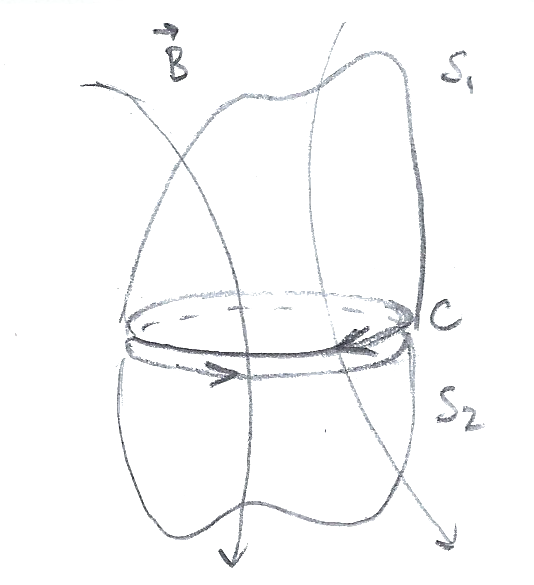
\includegraphics[scale=0.25]{images/em/faraday-surface.png}
\end{center}
First, let's look at how Faraday's Law is independent of the surface of which one calculates the flux. Consider a loop $C$ in space, and a surface $S_1$ bounded by the loop. We can apply the Faraday-Lenz Law:
\[
	\oint_C \vec E \cdot d\vec s = - \dv{}{t} \int_{S_1} \vec B \cdot \hat n \, dA
\]
Usually, we take loop integrals in the counterclockwise direction around the loop, but we can also consider a surface $S_2$ on the opposite side of the loop from $S_1$, from which we can apply Faraday-Lenz by integrating in the clockwise direction:
\[
	\oint_C \vec E \cdot d(-\vec s) = - \dv{}{t} \int_{S_2} \vec B \cdot \hat n \, dA
\]
Now, let's add these together. Notice the left side goes to 0, but when we combine the two flux integrals over surfaces $S_1$ and $S_2$, they form a closed surface. Because we assume Gauss' Law for Magnetism is true, this flux integral is 0!
\[
  - \dv{}{t} \int_{S_1} \vec B \cdot \hat n \, dA  - \dv{}{t} \int_{S_2} \vec B \cdot \hat n \, dA  = - \dv{}{t} \oint_{S_1+S_2} \vec B \cdot \hat n\, dA = -\dv{}{t} 0 = 0
\]
Because we haven't explicitly chosen a surface to take the magnetic flux through, Faraday-Lenz is independent upon the choice of the surface for the magnetic flux. However, let's look at Ampere's Law, which is not general for all cases (yet). \\
\begin{center}
	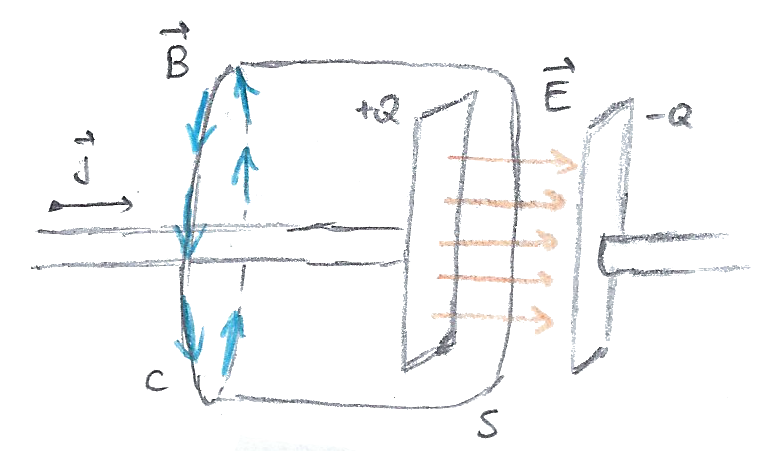
\includegraphics[scale=0.25]{images/em/ampere-capacitor.png}
\end{center}
Consider a straight wire connected to a parallel-plate capacitor:\\
We can apply Ampere's Law to the magnetic field in a circular loop $C$ with radius $r$ around the current running through the wire, and we know from the Magnetism unit that the magnetic field is non-zero. If we just consider the surface $S$ in the same plane as the loop, remember that we can derive the magnitude of the magnetic field:
\[
	\oint_C \vec B \cdot d\vec s = \mu_0 \int_S \vec j \cdot \hat n \, dA = \mu_0 I \rightarrow B \, 2\pi r = \mu_0 I \rightarrow B = \frac{\mu_0I}{2\pi r}
\]
What if we consider a surface $S$ that passes between the plates of the capacitor? No current runs between the plates of a capacitor, so then the right hand side of Ampere's Law goes to zero. However, the left-hand side of Ampere's Law we just saw to be nonzero! Something has gone horribly wrong...\\
Remember that the current charges the plates of the capacitor over time, creating an electric field in the capacitor. Maybe we should look at the electric field as it changes with time to see how we can still obtain the correct expression for the current in the wire from the electric field. Remember the electric field in a capacitor has magnitude $\frac{\sigma}{\epsilon_0}$, with $\sigma = \frac{Q}{A}$ as the charge density per unit area:
\[
	E = \frac{\sigma}{\epsilon_0} = \frac{Q}{A\epsilon_0}
\]
We can actually find the electric flux through the surface $S$! Since the electric field only penetrates through an area of $A$, we can find the electric flux $\Phi_E$ to be:
\[
	\Phi_E = EA = \frac{Q}{\epsilon_0}
\]
To find the current, we can isolate the charge, and take a time-derivative:
\[
	Q = \epsilon_0 EA = \epsilon_0 \Phi_E \rightarrow I = \dv{Q}{t} = \epsilon_0 \dv{\Phi_E}{t} = \epsilon_0 \dv{}{t} \int_S \vec E \cdot \hat n \, dA
\]
Notice that we now have a new expression for the current. If we just plugged this back into Ampere's Law, we could fix the problem! It turns out James Clark Maxwell figured he could do this, so we can write Ampere's Law (with Maxwell's correction):
\[
	\oint_C \vec B \cdot d\vec s = \mu_0 \left(\int_S \vec j \cdot \hat n \, dA + \epsilon_0  \dv{}{t} \int_S \vec E \cdot \hat n \, dA\right)
\]
This is the correct form of Ampere's Law. This added term is called the displacement current - even though it's not actually a current, it compensates so that it considers changing electric flux as "current" for surfaces that don't have any current through them. With this, we can show that Ampere-Maxwell's Law (what we're going to call the corrected form of Ampere's Law) is true for any surface, using the same tactic we used earlier for Faraday's Law. \\
\begin{center}
	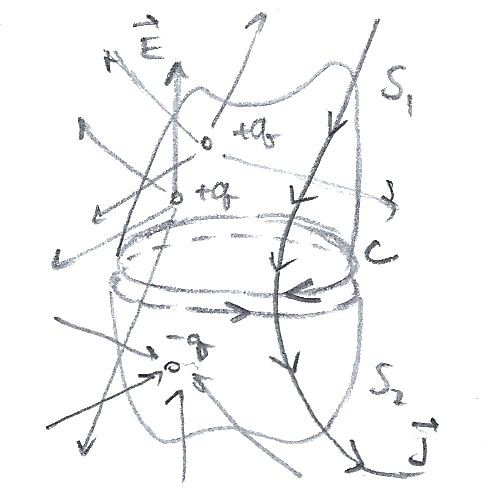
\includegraphics[scale=0.25]{images/em/ampere-surface.png}
\end{center}
Consider two surfaces $S_1$ and $S_2$ both bounded by a loop but on opposite sides of the loop. We can apply Ampere-Maxwell, but integrate both ways around the loop, attaining expressions pertaining to $S_1$ and $S_2$:
\[
	\oint_C \vec B \cdot d\vec s = \mu_0 \int_{S_1} \left(\vec j + \epsilon_0  \dv{}{t}\vec E\right) \cdot \hat n \, dA
\]	
\[
	\oint_C \vec B \cdot d(-\vec s) = \mu_0 \int_{S_2} \left(\vec j + \epsilon_0  \dv{}{t}\vec E\right) \cdot \hat n \, dA
\]
If we add them together, and consider the union of surfaces $S_1$ and $S_2$ into a single closed surface, we can simplify greatly:
\[
	\mu_0 \oint_{S_1+S_2} \vec j \cdot \hat n \, dA + \mu_0 \epsilon_0 \dv{}{t} \oint_{S_1+S_2} \vec E \cdot \hat n \, dA = 0
\]
We can apply Gauss' Law to the second term, and substitute in current $I_{out}$ for the first term:
\[
	\mu_0 I_{out} + \mu_0 \dv{Q_{inside}}{t} = 0
\]
In order for Ampere-Maxwell to be correct for any surface, if a net current flows out of a region, the charge inside the region must be changing at the same rate. This basically means that charge should be locally conserved, where the only way the charge inside a region can change is if a current explicitly carry it outside of the region. Local conservation of charge is actually a stronger statement than the conservation of charge, which only states that charge can neither be created nor destroyed. We actually just accept this to be true as a fundamental fact of the universe. \\
Because we know that charge is locally conserved, if we look back at the Lorentz Force Law:
\[
	\vec F = \dv{\vec P}{t} = q\vec E + q \vec v \times \vec B
\]
we can note that if charge is locally conserved, so should linear momentum be locally conserved - and for that matter, so should angular momentum and energy, the other two conserved quantities we discussed in mechanics. These three quantities can only change in a system if some form of their time derivatives, being force, torque, or power, change them over time. It seems like common sense, but we never said that there couldn't be a scenario where momentum or energy could just teleport from place to place before this point.\\
Regardless, we now have seen that Maxwell's equations now do apply in every scenario - and we can start to look at their applications in the next section, beyond how they describe everything that we know about electricity and magnetism.
\subsection{The Equations}
Just for the record, let's just state Maxwell's Equations explicitly, where $\rho$ is the density of charge per unit volume (being integrated over a volume) and $\vec j$ is the current density per unit area:
\begin{mdframed}[frametitle=Gauss' Law for Electric Fields]
	$$\oint_S \vec E \cdot \hat n \, dA = \frac{1}{\epsilon_0} \int_V \rho \, dV$$
\end{mdframed}
\begin{mdframed}[frametitle=Gauss' Law for Magnetic Fields]
	$$\oint_S \vec B \cdot \hat n \, dA = 0$$
\end{mdframed}
\begin{mdframed}[frametitle=Faraday-Lenz's Law of Induction]
	$$\oint_S \vec E \cdot d\vec s = -\dv{}{t} \int_S \vec B \cdot \hat n \, dA$$
\end{mdframed}
\begin{mdframed}[frametitle=Ampere-Maxwell's Circuital Law]
	$$\oint_S \vec B \cdot d\vec s = \mu_0 \int_S \left(\vec j + \epsilon_0  \dv{}{t}\vec E\right) \cdot \hat n \, dA$$
\end{mdframed}
Notice that how because of Faraday-Lenz's Law, a changing magnetic field induces an electric field, and because of Ampere-Maxwell's Law, a changing electric field also can create a magnetic field. This begs the question - are there such things as electric and magnetic fields that are self-sustaining? As in, is it possible to have an electric and magnetic field that keep creating more electric and magnetic fields to infinity? 
\begin{center}
	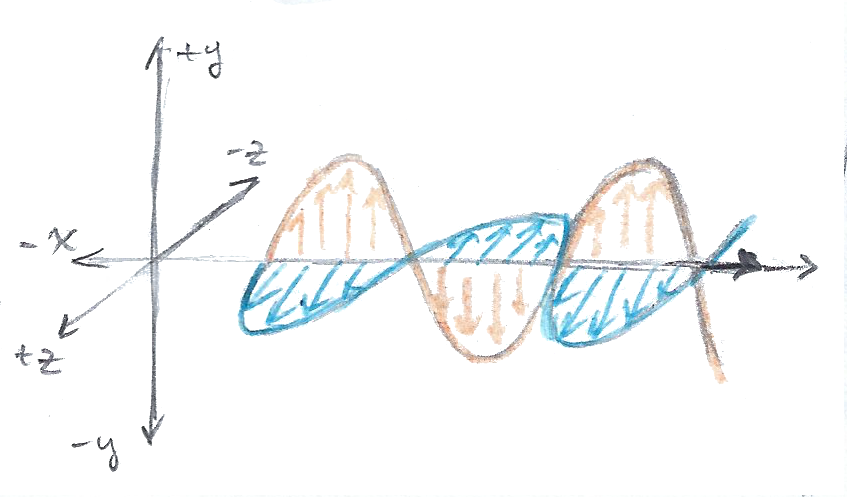
\includegraphics[scale=0.25]{images/em/em-waves.png}
\end{center}
The answer is yes, actually. If just consider free space, where there's no charge and no current, we can create a traveling wave of electric and magnetic fields that sustain each other. It can be shown that this is true and that the speed of this wave $c$ is
\[
	c = \frac{1}{\sqrt{\mu_0\epsilon_0}} = \frac{1}{\sqrt{1.257 \cdot 10^{-6} \, \text{H/m} \cdot 8.854 \cdot 10^{-12} \, \text{F/m}}} = 2.997 \cdot 10^{8} \, \text{m/s}
\]
You might recognize this as the speed of light $c$ in a vacuum - that's because it is. When Maxwell derived this result, he guessed that light itself was simply an electromagnetic wave, and this claim has been tested extensively and is accepted as true. \\